\documentclass{article}
\usepackage{graphicx} % Required for inserting images
\usepackage[binary-units]{siunitx}
\usepackage[utf8]{inputenc}
\usepackage{enumitem}
\usepackage{varwidth}
\usepackage{tikz}
\usepackage{circuitikz}
\usepackage{karnaugh-map}
\usepackage{tabularx}
\usepackage{siunitx}
\usepackage{circuitikz}
\usepackage{titlesec}
\usepackage{multirow}
\usepackage{pgf,tikz}
\usetikzlibrary{calc,arrows}
\usepackage{amsmath}
\usepackage{geometry}
\pagestyle{empty}

\title{GATE EC 2023}
\author{Mohiuddin}
\date{September 2023}
\begin{document}

\maketitle

\begin{enumerate}
\item In a given sequential circuit, initial states are $Q1 = 1$ and $Q2 = 0$. For a clock frequency of \SI{1}{\mega\hertz}, the frequency of signal $Q2$ in \si{\kilo\hertz}, is(rounded off to the nearest integer)
    
\begin{figure}[ht]
    \centering
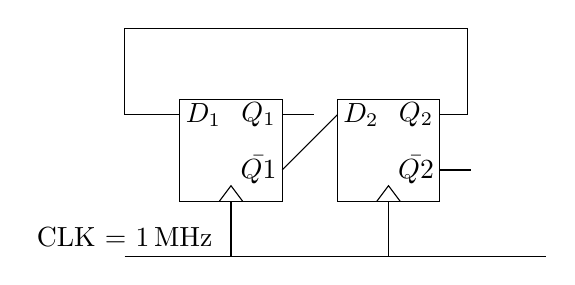
\begin{tikzpicture}          

% Drawing flip-flops
\draw (-1.3,-1.3) rectangle (0,0);
\draw(-1,-0.2) node{$D_1$};
\draw(-0.3,-0.2) node{$Q_1$};
\draw(-0.3,-0.9) node{$\Bar{Q1}$};

\draw(0.7,-1.3) rectangle (2,0);
\draw(1,-0.2) node{$D_2$};
\draw(1.7,-0.2) node{$Q_2$};
\draw(1.7,-0.9) node{$\Bar{Q2}$};

% Connecting them
\draw(0,-0.9) -- (0.7,-0.2);
\draw(0,-0.2) -- (0.4,-0.2);
\draw(2,-0.2) -- (2.35,-0.2);
\draw(2.0,-0.9) -- (2.4,-0.9);


% Drawing clk
\draw(-2,-2) node[above]{CLK = \SI{1}{\mega\hertz} } -- (3.35,-2);

% Connecting clk
\draw(-0.65,-2) -- (-0.65,-1.3);
\draw(1.35,-2) -- (1.35,-1.3);

% Drawing clk edges
\draw(-0.5,-1.3) -- (-0.65,-1.1) -- (-0.8,-1.3);
\draw(1.2,-1.3) -- (1.35,-1.1) -- (1.5,-1.3);

% Drawing Q2, D1,
\draw(2.35,-0.2) --(2.35,0.9);
\draw(2.35,0.9) -- (-2,0.9);
\draw(-2,0.9)--(-2.0,-0.2);
\draw(-2,-0.2)--(-1.3,-0.2);


\end{tikzpicture}
\end{figure}
\end{enumerate}
\end{document}
